\documentclass[aspectratio=169]{beamer}

\usetheme{Madrid}
\usecolortheme{seahorse}

\usepackage{listings}
\usepackage{xcolor}
\usepackage{graphicx}
\usepackage{tikz}
\usepackage{fontawesome5}
\usepackage{tcolorbox}

% Custom colors
\definecolor{claudepurple}{RGB}{114, 92, 214}
\definecolor{claudelight}{RGB}{243, 240, 255}
\definecolor{termgreen}{RGB}{0, 200, 83}
\definecolor{termbg}{RGB}{30, 30, 30}

% Code listing style
\lstset{
    basicstyle=\ttfamily\small,
    backgroundcolor=\color{claudelight},
    frame=single,
    framerule=0pt,
    breaklines=true,
    columns=fullflexible,
    keepspaces=true,
}

% Terminal style
\newtcolorbox{terminal}{
    colback=termbg,
    colframe=termbg,
    coltext=white,
    fontupper=\ttfamily\small,
    arc=4pt,
    boxrule=0pt,
}

% Prompt box style
\newtcolorbox{promptbox}{
    colback=claudelight,
    colframe=claudepurple,
    fontupper=\normalfont,
    arc=4pt,
    boxrule=1pt,
    left=8pt,
    right=8pt,
    top=6pt,
    bottom=6pt,
}

% Question box style (for interactive elements)
\newtcolorbox{questionbox}{
    colback=white,
    colframe=claudepurple,
    fontupper=\normalfont\small,
    arc=4pt,
    boxrule=1.5pt,
    left=8pt,
    right=8pt,
    top=6pt,
    bottom=6pt,
    title={\faIcon{question-circle} Claude is asking...},
    fonttitle=\bfseries\color{claudepurple},
    coltitle=claudepurple,
    attach boxed title to top left={yshift=-2mm,xshift=4mm},
    boxed title style={colback=white,colframe=white},
}

\setbeamercolor{frametitle}{fg=claudepurple}
\setbeamercolor{title}{fg=claudepurple}
\setbeamercolor{structure}{fg=claudepurple}

\title{Building with Claude Code}
\subtitle{From Simple Tasks to Research-Scale Projects}
\author{MGMT 408 -- UCLA Anderson}
\date{\today}
\institute{UCLA Anderson School of Management}

\begin{document}

% Title slide
\begin{frame}
    \titlepage
\end{frame}

% Outline
\begin{frame}{Outline}
    \tableofcontents
\end{frame}

% ============================================================================
\section{What is Claude Code?}
% ============================================================================

\begin{frame}{What is Claude Code?}
    \begin{columns}
        \begin{column}{0.6\textwidth}
            \textbf{Claude Code} is Anthropic's agentic coding tool that:
            \vspace{0.5em}
            \begin{itemize}
                \item Runs in your terminal alongside your codebase
                \item Reads, writes, and edits files directly
                \item Executes shell commands (git, npm, python, etc.)
                \item Browses documentation and searches the web
                \item Maintains context across an entire session
                \item \textbf{Asks clarifying questions} when needed
            \end{itemize}
            \vspace{0.5em}
            Unlike ChatGPT: Claude Code \textit{operates} on your project, not just \textit{discusses} it.
        \end{column}
        \begin{column}{0.35\textwidth}
            \begin{terminal}
\$ claude

\textcolor{termgreen}{>} What would you like to work on?

\textcolor{gray}{I can read your files, run}
\textcolor{gray}{commands, and help you build.}
            \end{terminal}
        \end{column}
    \end{columns}
\end{frame}

\begin{frame}{How It Works: The Agentic Loop}
    \begin{center}
        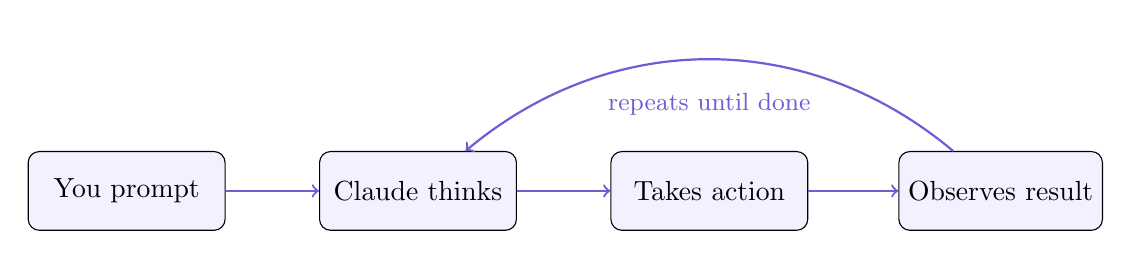
\begin{tikzpicture}[node distance=2.2cm, auto]
            \node[draw, rounded corners, fill=claudelight, minimum width=2.5cm, minimum height=1cm] (prompt) {You prompt};
            \node[draw, rounded corners, fill=claudelight, minimum width=2.5cm, minimum height=1cm, right of=prompt, xshift=1.5cm] (think) {Claude thinks};
            \node[draw, rounded corners, fill=claudelight, minimum width=2.5cm, minimum height=1cm, right of=think, xshift=1.5cm] (act) {Takes action};
            \node[draw, rounded corners, fill=claudelight, minimum width=2.5cm, minimum height=1cm, right of=act, xshift=1.5cm] (observe) {Observes result};

            \draw[->, thick, claudepurple] (prompt) -- (think);
            \draw[->, thick, claudepurple] (think) -- (act);
            \draw[->, thick, claudepurple] (act) -- (observe);
            \draw[->, thick, claudepurple] (observe) to[bend right=40] node[below, yshift=-0.3cm] {\small repeats until done} (think);
        \end{tikzpicture}
    \end{center}

    \vspace{1em}
    \textbf{Actions include:}
    \begin{itemize}
        \item \texttt{Read} -- examine files in your project
        \item \texttt{Write/Edit} -- create or modify code
        \item \texttt{Bash} -- run terminal commands
        \item \texttt{WebFetch} -- retrieve documentation
        \item \texttt{AskUserQuestion} -- request clarification from you
    \end{itemize}
\end{frame}

% ============================================================================
\section{Case Study: Finance Practice Tool}
% ============================================================================

\begin{frame}{The Task: Build a Practice Tool}
    \textbf{Starting point:} PDF lecture slides for MGMT 408 (Foundations of Finance)

    \vspace{1em}
    \textbf{Goal:} Create an interactive web-based practice tool with:
    \begin{itemize}
        \item 40 practice problems across 4 topics (TVM, Capital Budgeting, Stocks, Bonds)
        \item Adaptive hints (3 levels) and full solutions
        \item Built-in calculator
        \item Progress tracking with localStorage
        \item 2 practice midterms (40 multiple-choice questions)
        \item LaTeX formula rendering
    \end{itemize}

    \vspace{1em}
    \textbf{Result:} 8 HTML files, ~3,200 lines of code

    \vspace{0.5em}
    \textit{Built entirely through natural language conversation with Claude Code.}
\end{frame}

\begin{frame}[fragile]{Prompt \#1: Initial Request}
    \begin{promptbox}
        \textbf{User:} \\[0.3em]
        ``I uploaded my finance lecture slides. Can you create a web-based practice tool with problems similar to what's covered in the slides? Include a calculator and hint system.''
    \end{promptbox}

    \vspace{1em}
    \textbf{What Claude Code did:}
    \begin{enumerate}
        \item Read the uploaded PDF slides
        \item Identified key topics (TVM, NPV, stock valuation, bonds)
        \item Generated 40 problems with solutions
        \item Built responsive HTML/CSS/JS interface
        \item Added scientific calculator component
        \item Implemented 3-level hint system
    \end{enumerate}

    \vspace{0.5em}
    \textcolor{gray}{\small No manual coding required -- Claude wrote, tested, and iterated autonomously.}
\end{frame}

\begin{frame}{Interactive Clarification}
    When Claude needed decisions, it asked:

    \vspace{0.5em}
    \begin{questionbox}
        \textbf{What format would you like for the slides?}

        \vspace{0.3em}
        \begin{itemize}
            \item[$\circ$] Google Slides -- \textit{I'll provide content you can copy}
            \item[$\circ$] PowerPoint -- \textit{I'll create a .pptx file}
            \item[$\bullet$] \textbf{PDF/Beamer} -- \textit{Code-based slides in LaTeX}
            \item[$\circ$] Markdown/reveal.js -- \textit{Browser-based slides}
        \end{itemize}

        \vspace{0.5em}
        \textbf{What's the target audience?}

        \vspace{0.3em}
        \begin{itemize}
            \item[$\circ$] Technical (CS/Engineering)
            \item[$\circ$] Business/MBA students
            \item[$\circ$] General university audience
            \item[$\bullet$] \textbf{Faculty/researchers}
        \end{itemize}
    \end{questionbox}

    \vspace{0.5em}
    \textcolor{gray}{\small This prevents wasted effort and ensures the output matches your needs.}
\end{frame}

\begin{frame}[fragile]{Prompt \#2: Code Review}
    \begin{promptbox}
        \textbf{User:} \\[0.3em]
        ``Can you explain what this does so far?''
    \end{promptbox}

    \vspace{0.5em}
    \textbf{Claude's response:} A structured analysis of the codebase:

    \begin{terminal}
\textcolor{termgreen}{Structure:} 8 HTML files (~6,765 lines)

| File               | Purpose                    |
|--------------------|----------------------------|
| index.html         | Landing page / navigation  |
| week1-tvm.html     | Time Value of Money (10)   |
| week2-capbudget.html | Capital Budgeting (10)   |
| week3-stocks.html  | Stock Valuation (10)       |
| week4-bonds.html   | Bond Valuation (10)        |
| midterm1.html      | Practice Exam 1 (20 MCQ)   |
| midterm2.html      | Practice Exam 2 (20 MCQ)   |
    \end{terminal}
\end{frame}

\begin{frame}[fragile]{Prompt \#3: Improvement Suggestions}
    \begin{promptbox}
        \textbf{User:} \\[0.3em]
        ``Do you have suggestions to improve this?''
    \end{promptbox}

    \vspace{0.5em}
    Claude identified 14 specific issues, prioritized by impact:

    \begin{enumerate}
        \item \textbf{Code duplication} -- 3,400 lines of CSS/JS repeated across 4 files
        \item \textbf{localStorage broken} -- progress tracking never saved
        \item \textbf{KaTeX not rendering} -- \texttt{renderMath()} was a no-op
        \item Calculator uses \texttt{eval()} -- minor security concern
        \item No question randomization
        \item Missing accessibility features
        \item \textit{...and 8 more}
    \end{enumerate}

    \vspace{0.5em}
    \textcolor{gray}{\small Claude doesn't just build -- it reviews, critiques, and suggests improvements.}
\end{frame}

\begin{frame}[fragile]{Prompt \#4: Implement Fixes}
    \begin{promptbox}
        \textbf{User:} \\[0.3em]
        ``sure'' \textcolor{gray}{(in response to ``Want me to implement any of these?'')}
    \end{promptbox}

    \vspace{0.5em}
    Claude autonomously:
    \begin{itemize}
        \item Created \texttt{practice.css} (shared styles)
        \item Created \texttt{practice.js} (shared logic + localStorage + KaTeX fix)
        \item Refactored all 4 weekly pages to use shared files
        \item Updated LaTeX formulas to proper syntax
        \item Committed changes with descriptive message
        \item Pushed to GitHub
    \end{itemize}

    \vspace{0.5em}
    \begin{terminal}
\textcolor{termgreen}{Result:} 6 files changed
         882 insertions(+), 3,385 deletions(-)

         Net: \textbf{2,500 lines removed} (deduplication)
    \end{terminal}
\end{frame}

\begin{frame}[fragile]{Prompt \#5: Verification}
    \begin{promptbox}
        \textbf{User:} \\[0.3em]
        ``Can you visit the website and make sure it is all working as intended?''
    \end{promptbox}

    \vspace{0.5em}
    Claude ran a comprehensive test suite:
    \begin{itemize}
        \item Started local HTTP server
        \item Verified all 10 files return HTTP 200
        \item Checked 16 required DOM elements in each page
        \item Validated JavaScript syntax
        \item Verified all 40 problems have required fields
        \item Tested cross-page navigation links
    \end{itemize}

    \vspace{0.5em}
    \begin{terminal}
=== week1-tvm.html ===
  topicKey: tvm
  Problem count: 10
  All fields OK

\textcolor{termgreen}{All pages validated successfully.}
    \end{terminal}
\end{frame}

% ============================================================================
\section{The CLAUDE.md File}
% ============================================================================

\begin{frame}[fragile]{Project Memory: CLAUDE.md}
    Claude Code reads a \texttt{CLAUDE.md} file in your repo root to understand project context:

    \vspace{0.5em}
    \begin{lstlisting}[language={}]
# Finance Practice Tool

## Project Structure
- index.html: Main landing page
- week{1-4}-*.html: Practice problem pages
- midterm{1,2}.html: Exam simulations
- practice.css/js: Shared code

## Tech Stack
- Pure HTML/CSS/JS (no framework)
- KaTeX for LaTeX rendering
- localStorage for progress tracking

## Development Notes
- Problems are embedded as JS arrays
- Each problem needs: id, topic, difficulty,
  problem_text, formula, solution_steps,
  correct_answer, hints (3 levels)
    \end{lstlisting}
\end{frame}

\begin{frame}{Why CLAUDE.md Matters}
    \textbf{Without CLAUDE.md:}
    \begin{itemize}
        \item Claude must re-explore the codebase each session
        \item May make inconsistent architectural decisions
        \item Loses track of project conventions
    \end{itemize}

    \vspace{1em}
    \textbf{With CLAUDE.md:}
    \begin{itemize}
        \item Instant context on project structure
        \item Consistent coding style across sessions
        \item Remembers key decisions (``no frameworks'', ``problems need 3 hint levels'')
        \item Can include TODOs, known issues, deployment notes
    \end{itemize}

    \vspace{1em}
    \textcolor{claudepurple}{\textbf{Think of it as onboarding documentation for your AI collaborator.}}
\end{frame}

% ============================================================================
\section{Applications for Research}
% ============================================================================

\begin{frame}{Scaling to Research Projects}
    The same workflow applies to larger, research-scale tasks:

    \vspace{1em}
    \begin{columns}
        \begin{column}{0.48\textwidth}
            \textbf{Data Analysis}
            \begin{itemize}
                \item Parse and clean datasets
                \item Run statistical analyses
                \item Generate publication-ready figures
                \item Iterate on methodology
            \end{itemize}
        \end{column}
        \begin{column}{0.48\textwidth}
            \textbf{Literature \& Writing}
            \begin{itemize}
                \item Search and summarize papers
                \item Draft methodology sections
                \item Format citations
                \item Convert between formats
            \end{itemize}
        \end{column}
    \end{columns}

    \vspace{1em}
    \begin{columns}
        \begin{column}{0.48\textwidth}
            \textbf{Experiment Infrastructure}
            \begin{itemize}
                \item Build survey tools (like this one)
                \item Create participant interfaces
                \item Log and process results
            \end{itemize}
        \end{column}
        \begin{column}{0.48\textwidth}
            \textbf{Reproducibility}
            \begin{itemize}
                \item Generate Docker configs
                \item Write setup documentation
                \item Create replication packages
            \end{itemize}
        \end{column}
    \end{columns}
\end{frame}

\begin{frame}{Key Advantages for Researchers}
    \begin{enumerate}
        \item \textbf{Reduces context-switching} \\
        Stay in natural language; Claude handles the implementation details

        \vspace{0.5em}
        \item \textbf{Handles tedious tasks} \\
        Data cleaning, formatting, boilerplate code -- delegate confidently

        \vspace{0.5em}
        \item \textbf{Catches errors proactively} \\
        Reviews its own work, runs tests, validates outputs

        \vspace{0.5em}
        \item \textbf{Documents as it goes} \\
        Commit messages, code comments, CLAUDE.md updates

        \vspace{0.5em}
        \item \textbf{Learns your project} \\
        Maintains context across long sessions; CLAUDE.md persists across sessions
    \end{enumerate}
\end{frame}

% ============================================================================
\section{Getting Started}
% ============================================================================

\begin{frame}[fragile]{Getting Started}
    \textbf{Installation:}
    \begin{terminal}
npm install -g @anthropic-ai/claude-code
    \end{terminal}

    \vspace{0.5em}
    \textbf{Usage:}
    \begin{terminal}
cd your-project
claude
    \end{terminal}

    \vspace{1em}
    \textbf{Tips for effective use:}
    \begin{itemize}
        \item Start with a clear, specific request
        \item Let Claude ask clarifying questions (don't over-specify upfront)
        \item Review outputs and provide feedback
        \item Create a \texttt{CLAUDE.md} for ongoing projects
        \item Use Git -- Claude commits its work
    \end{itemize}

    \vspace{1em}
    \textcolor{claudepurple}{\textbf{Docs:} \texttt{https://docs.anthropic.com/claude-code}}
\end{frame}

\begin{frame}{}
    \begin{center}
        \Huge\textcolor{claudepurple}{Questions?}

        \vspace{2em}
        \large
        Finance Practice Tool: \texttt{github.com/[your-repo]}

        \vspace{0.5em}
        Claude Code: \texttt{anthropic.com/claude-code}
    \end{center}
\end{frame}

\end{document}
